\section{Theory}

Solar cells, also known as photovoltaic (PV) cells can convert sunlight directly into electricity using
the photovoltaic effect. 
This technology is widely used in satellites, power
grids, and renewable energy solutions, with research fo-
cusing on efficiency, cost reduction, and integration into
everyday applications such as electric vehicles and smart
grids.

The fundamental working principle of these cells are based on the behavior of p-n junction diodes. 
At the p-n junction, electrons from the n-type region diffuse towards the
p-type region, while holes from the p-type region move
toward the n-type region. This diffusion process exposes
positively charged ion cores in the n-region and negatively charged ion cores in the p-region, leading to the
formation of an electric field across the junction. This potential barrier is known as the depletion region.

When sunlight
strikes the surface of a solar cell, photons with energy greater than the band gap energy of the semiconductor material excite
electrons from the valence band to the conduction band. These electron-hole pairs are then separated due to the existing potential barrier, creating a potential difference
across the solar cell, similar to a battery.

\begin{figure}
    \centering
    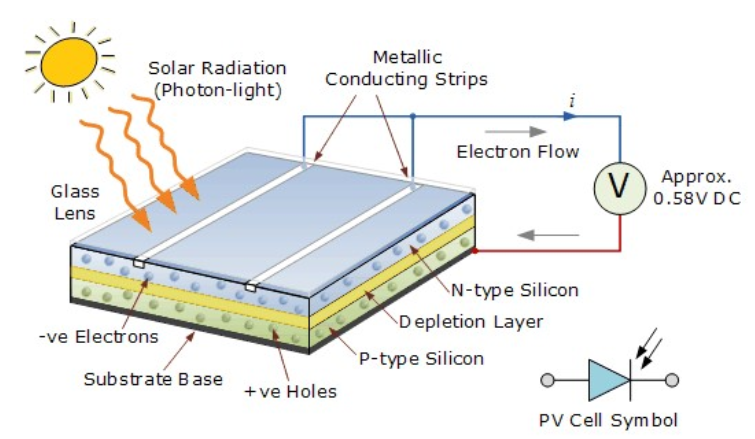
\includegraphics[width=1\columnwidth]{images/scheme.png}
    \caption{Parts of a Solar Cell}
\end{figure}

A solar cell typically consists of the following key com-
ponents:\\

\begin{itemize}
    \item \textbf{Front Contact:} A transparent conductive layer
    (usually made of materials like indium tin oxide)
    that allows sunlight to pass through while also conducting the generated current.
    \item \textbf{p-n Junction:} The heart of the solar cell, where
    the p-type and n-type semiconductors meet. This
    junction creates an electric field that helps in the
    separation of electron-hole pairs generated by the
    absorbed sunlight.
    that allows sunlight to pass through while also conducting the generated current.
    \item \textbf{Absorber Layer:} This is where the majority of
    sunlight is absorbed to generate electron-hole pairs.
    Silicon is commonly used in this layer due to its
    effective light-absorbing properties.
    \item \textbf{Back Contact:} A conductive layer at the rear of
    the cell that completes the electrical circuit, allowing electrons to return after passing through the
    external load.\\
\end{itemize}

Additionally, to enhance efficiency, modern solar cells
incorporate anti-reflective coatings to minimize light loss,
passivation layers to reduce recombination, and multijunction structures that utilize different semiconductor
materials to capture a broader range of the solar spectrum.

Mathematically, the diode equation is expressed as:

\begin{align}
    I = I_0 \left(e^\frac{qV}{nk_B T} - 1\right) - I_L
\end{align}

where, $I_0$ is the dark saturation current (leakage current
in the absence of light), $q$ is the charge of an electron, $V$ is the applied voltage,
$k_B$ is the Boltzmann constant, $T$ is the absolute temperature, $I_L$ is the light generated current (The additional currentproduced due to photon absorption, which enhances the overall current output) and $n$ is the ideality factor (a measure of how closely the diode follows the ideal diode equation).

\begin{figure}
    \centering
    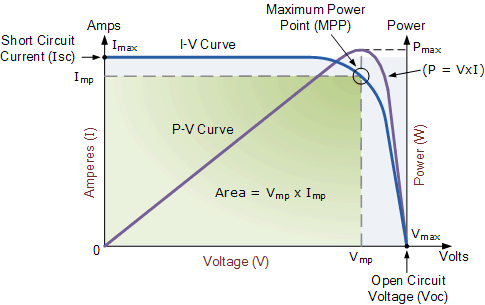
\includegraphics[width=1\columnwidth]{images/curve.png}
    \caption{Typical I-V and power curves of a solar cell}
\end{figure}

The performance of a solar cell is measured by the following parameters:\\

\begin{itemize}
    \item \textbf{Short-Circuit Current ($I_\text{sc}$):} The maximum current generated when the solar cell is short-circuited
    (V = 0). It depends on the intensity of incident
    light and the material properties of the cell.
    \item \textbf{Open Circuit Voltage ($V_\text{oc}$):} The maximum voltage produced when no current flows (I = 0). It is
    influenced by the semiconductor material and temperature.
    \item \textbf{Fill Factor ($FF$):} A measure of how `square' the
    I-V curve appears, defined as:
    \begin{align}
        FF = \frac{V_\text{mp}I_\text{mp}}{V_\text{oc}I_\text{oc}}
    \end{align}
    where $V_\text{mp}$ and $I_\text{mp}$ are the voltage and current at maximum power output, respectively.
    \item \textbf{Efficiency ($\eta$):} The ratio of the electrical output
    power to the incident solar power, expressed as:
    \begin{align}
        \eta = \frac{P_\text{max}}{P_\text{in}} = \frac{V_\text{oc} I_\text{sc} \cdot FF}{P_\text{in}}
    \end{align}
    where $P_\text{in}$ denotes the incident light power per unit
area. The efficiency is influenced by light intensity,
temperature, and the material properties of the solar cell.
    
\end{itemize}
% ======================================================================================
\section{Experimental Setup}

\subsection*{Apparatus}

\begin{enumerate}
    \item Solar cell
    \item Potentiometer
    \item Optical filter papers
    \item Multimeters
    \item Incandescent lamp 
    \item Connecting wires\\
\end{enumerate}

A circuit diagram of the experimental setup is illustrated in Figure \ref{circuit}. A potentiometer is employed to vary the resistance within
the circuit, allowing for controlled adjustment of the load.
A multimeter is connected in series with the solar cell
to measure the current (I), while a second multimeter is
connected in parallel to measure the voltage (V) across
the solar cell. Now we use this to analyze the
impact of different light intensities and wavelengths on the performance of the solar cell under both incandescent light and sunlight.

\begin{figure}[H]
    \centering
    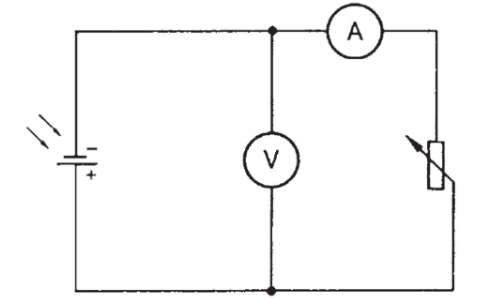
\includegraphics[width=0.7\columnwidth]{images/circuit.png}
    \caption{Circuit diagram of the experimental setup}
    \label{circuit}
\end{figure}